\documentclass[11pt]{article}
\usepackage[margin=1in]{geometry}
\usepackage{graphicx}
\usepackage{booktabs}
\usepackage{amsmath}
\usepackage{amssymb}
\usepackage[T1]{fontenc}
\usepackage{helvet}                     % Helvetica for the sans-serif title/headings
\usepackage{natbib}
\usepackage{xcolor}
\definecolor{linkblue}{HTML}{2A5DB0}
\definecolor{boxgray}{HTML}{F0F2F5}
\usepackage[colorlinks=true,citecolor=linkblue,linkcolor=linkblue,urlcolor=linkblue]{hyperref}

% --- Meta-FAIR-style headings: sans-serif, bold (base LaTeX \@startsection, no extra packages) ---
\makeatletter
\renewcommand\section{\@startsection{section}{1}{\z@}%
  {-3.5ex \@plus -1ex \@minus -.2ex}{2.0ex \@plus.2ex}%
  {\normalfont\large\sffamily\bfseries}}
\renewcommand\subsection{\@startsection{subsection}{2}{\z@}%
  {-2.5ex\@plus -1ex \@minus -.2ex}{1.2ex \@plus .2ex}%
  {\normalfont\normalsize\sffamily\bfseries}}
\renewcommand\paragraph{\@startsection{paragraph}{4}{\z@}%
  {1.6ex \@plus1ex \@minus.2ex}{-0.6em}%
  {\normalfont\normalsize\sffamily\bfseries}}
\makeatother
\setlength{\parindent}{0pt}
\setlength{\parskip}{0.5em}

% Gray rounded-ish abstract box (base LaTeX: colorbox + minipage)
\newcommand{\abstractbox}[1]{%
  \begingroup\setlength{\fboxsep}{10pt}%
  \noindent\colorbox{boxgray}{\begin{minipage}{\dimexpr\textwidth-2\fboxsep\relax}#1\end{minipage}}%
  \endgroup}

\begin{document}

% --- Title block (left-aligned, sans-serif, bold — Meta FAIR style) ---
\begin{flushleft}
{\sffamily\bfseries\fontsize{20}{24}\selectfont
A global predicted-fMRI drive signal from TRIBE does not predict YouTube replay heatmaps\par}
\vspace{10pt}
\begin{tabular}[t]{@{}l@{\hskip 3.5em}l@{}}
{\sffamily\bfseries Barada Sahu} & {\sffamily\bfseries Shivesh Pandey}\\[1pt]
Cabal AI & Para AI
\end{tabular}
\end{flushleft}

% --- Abstract in a gray box (Meta FAIR style, no "Abstract" heading) ---
\abstractbox{%
Deep multimodal brain-encoding models predict fMRI responses to naturalistic video accurately
enough to ask a further question: do their \emph{predicted} neural signals also forecast
real-world behavioral engagement? We test this at scale. We run TRIBE, the winning model of the
2025 Algonauts brain-encoding challenge (Llama-3.2 + V-JEPA2 + Wav2Vec-BERT), on YouTube videos,
derive a per-second predicted-engagement curve (the global field power of the predicted cortical
response), and correlate it against each video's crowd-sourced ``most replayed'' heatmap, a
passively-collected proxy for which moments viewers return to. Across 48 videos spanning 11
content categories, this signal shows no evidence of predicting re-watch behavior: the pooled
position-controlled partial correlation is $+0.058$ (95\% CI $[-0.04, 0.15]$; one-sample
$t(47)=1.21$, $p=0.23$), indistinguishable from zero, and it does not exceed simple low-level
baselines (audio loudness $+0.04$, paired $p=0.74$; visual motion $-0.06$). Even the raw
correlation is $\approx 0$ on this set; the moderate raw correlations obtained for music videos
are a genre-specific intro/onset-replay artifact that does not generalize. For the most-replayed
target and a global-field-power readout, predicted-fMRI engagement does not predict re-watch
behavior beyond temporal position and low-level audiovisual features. We release the full pipeline,
including an acquisition method that works despite YouTube's SABR-only streaming.

\vspace{4pt}
\textbf{Date:}~\today \\
\textbf{Correspondence:}~\texttt{barada@gmail.com}, \texttt{cs21bt067.alum25@iitdh.ac.in}
}

\vspace{6pt}

\section{Introduction}
Encoding models that predict brain activity from naturalistic stimuli have improved sharply, with
deep multimodal architectures such as TRIBE winning the 2025 Algonauts challenge (out of 263 teams)
by mapping fused text, video, and audio features onto the cortical surface~\citep{dascoli2025tribe}.
Separately, the \emph{neuroforecasting} literature shows that \emph{measured} neural signals
(fMRI/EEG) can predict aggregate population behavior beyond self-report, from cultural
popularity~\citep{berns2012neural} to crowdfunding and market outcomes~\citep{genevsky2017brain},
and that the temporal reliability of neural processing tracks audience
preferences~\citep{dmochowski2014audience,hasson2004intersubject}.

Whether \emph{predicted} neural signals, which need no scanner and are cheap to compute, inherit
this predictive power has not been tested. We provide the first evaluation of a predicted-fMRI
engagement signal against a large, passively-collected behavioral target: YouTube's ``most
replayed'' heatmaps. We contribute (i)~a method to turn TRIBE predictions into a per-second
engagement curve and evaluate it against most-replayed; (ii)~a position-controlled and baseline-controlled
evaluation across a category-diverse sample; (iii)~a reproducible null result; and (iv)~an
acquisition and scoring pipeline we release, including a workaround for YouTube's SABR-only
streaming.

\section{Related Work}
\paragraph{Brain encoding of naturalistic stimuli.} Voxel-wise and surface-based encoding models
predict fMRI responses to video/audio/text; TRIBE fuses Llama-3.2~\citep{grattafiori2024llama},
V-JEPA2~\citep{bardes2024vjepa}, and Wav2Vec-BERT features and predicts per-TR responses on the
\texttt{fsaverage5} surface~\citep{dascoli2025tribe}.
\paragraph{Neuroforecasting.} Measured neural signals predict behavioral and market outcomes beyond
stated preference~\citep{berns2012neural,genevsky2017brain}; neural reliability across viewers
predicts engagement~\citep{dmochowski2014audience}. A reason to expect this to transfer to
\emph{predicted} signals is that an encoding model trained to reproduce cortical responses should,
if accurate, reproduce whatever behaviorally-relevant structure those responses carry. Two reasons
to doubt it: the neuroforecasting effect is often carried by individual variability and
region-specific reward/salience activity that group-trained encoders regress toward the mean and a
whole-cortex readout discards; and a model optimized for average fMRI accuracy is not optimized to
preserve the moment-to-moment contrasts that drive re-watching. Which effect dominates is an
empirical question, and the one we test.
\paragraph{Engagement prediction.} Video ``highlight'' and engagement models typically use
low-level audiovisual features; ``most replayed'' is a large but biased target (intro/onset
effects, chapter markers, seek-back behavior), which motivates our position and baseline controls.

\section{Method}
\subsection{Model}
TRIBE~\citep{dascoli2025tribe} is a 1B-parameter trimodal encoder trained on $500{+}$ hours of
fMRI from $700{+}$ individuals. It extracts features from three frozen foundation encoders
(Llama-3.2~\citep{grattafiori2024llama} over the dialogue transcript, V-JEPA2~\citep{bardes2024vjepa}
over video frames, and Wav2Vec-BERT over the soundtrack), temporally aligns them, and fuses them
with a Transformer conditioned on a learned subject embedding to predict the per-TR cortical
response $\mathbf{P}\in\mathbb{R}^{T\times V}$ on the \texttt{fsaverage5} surface
($V{=}20{,}484$ vertices, TR${=}1$\,s). We use the released weights with no fine-tuning; because we
study relative temporal dynamics, we average over subject embeddings and analyze the resulting
predicted response.

\subsection{Engagement readout}
We summarize the high-dimensional prediction into a scalar per-TR \emph{engagement} value via the
\emph{global field power} (GFP), the root-mean-square over vertices,
\begin{equation}
e_t=\sqrt{\tfrac{1}{V}\textstyle\sum_{v=1}^{V} P_{t,v}^2},\qquad t=1,\dots,T .
\end{equation}
GFP indexes how strongly the stimulus drives the cortex overall and makes no assumption about
which regions matter. We take it as a candidate engagement signal and test that interpretation
rather than assume it; the region-restricted variants in \S\ref{sec:region} relax the
whole-cortex assumption. Each TR is placed on the true video timeline using the model's segment
onsets, and we retain the first $60$\,s ($\approx 60$ TRs) per video.

\subsection{Behavioral target}
YouTube's ``most replayed'' heatmap reports $100$ markers per video, each a normalized
re-watch intensity in $[0,1]$ (relative to the video's peak). We linearly interpolate the marker
series onto the model's TR grid to obtain a target $g_t$ commensurate with $e_t$.

\subsection{Correlation and position control}
The raw association is the Pearson correlation $r_{\text{raw}}=\mathrm{corr}(e,g)$. Because both the
engagement curve and most-replayed carry a strong low-order temporal trend (intros and onsets are
re-watched, and predicted response often decays over a clip), $r_{\text{raw}}$ conflates
\emph{content} with \emph{position}. We therefore use as the primary metric the
\emph{position-controlled partial correlation}: we regress each series on a position basis
$\mathbf{B}=[\mathbf{1},\,t,\,t^2]$ by ordinary least squares and correlate the residuals,
\begin{equation}
r_{\text{part}}=\mathrm{corr}\big(e-\mathbf{B}\hat{\beta}_e,\; g-\mathbf{B}\hat{\beta}_g\big).
\end{equation}
The quadratic basis removes the dominant monotone-plus-onset trend without overfitting $\sim\!60$
points, isolating whether $e$ tracks $g$ at the level of \emph{which specific moments} are
re-watched.

\subsection{Pooling and inference}
Each video yields one $r_{\text{part},i}$. We report the unweighted mean across videos (equivalent
to Fisher-$z$ pooling here, and avoids over-weighting longer clips), test it against zero with a
one-sample $t$-test and a sign test, and compare it to each baseline with a paired $t$-test. We
report 95\% confidence intervals from the between-video standard deviation.

\subsection{Low-level baselines}
To calibrate any observed effect, we compute two content-derived control curves and pass them
through the identical raw/partial pipeline: \emph{loudness}, the per-second RMS energy of the
mono $16$\,kHz waveform; and \emph{motion}, the mean absolute frame-to-frame pixel difference of
$1$\,fps, $64{\times}36$ grayscale frames. TRIBE is deemed predictive only if $r_{\text{part}}$
clearly exceeds these.

\section{System and Pipeline}
A practical contribution of this work is an end-to-end pipeline that makes the study feasible and
fully reproducible despite two obstacles: YouTube's anti-download measures and the cost of encoding.

\paragraph{Acquisition under SABR.} As of 2025 YouTube serves most popular videos via SABR
(server-side adaptive bitrate) streaming, which exposes no directly downloadable media; standard
tools (yt-dlp, youtube-dl, cobalt) return only storyboard images or fail, on both residential and
datacenter IPs. We instead acquire videos with the NewPipe Android client running on a physical
device, driven programmatically over ADB with UI-automation, which succeeds where those tools fail.
The behavioral target is unaffected: most-replayed heatmaps are metadata and are fetched separately
without downloading media.

\paragraph{Encoding cache.} Encoding is the dominant cost ($\sim\!6$--$13$ minutes of GPU per clip,
driven by V-JEPA2). We cache the model output $\mathbf{P}$ (and per-TR onsets) on a network volume,
keyed by video and analysis window, so that no video is re-encoded across runs or re-analyses;
downstream readouts, baselines, and statistics are cheap CPU operations recomputed on demand.

\paragraph{Resumable, connectivity-independent scoring.} Scoring runs as a deployed serverless
function that fans out one video per GPU worker, each reading its clip from the volume; every
per-video result is committed immediately, so the study is resumable and survives client
disconnects, and a GPU-free aggregation step pools the cached results incrementally as they land.

\section{Experiments}
We analyze $N=48$ videos with most-replayed heatmaps spanning $11$ categories (music~17, talk~5,
tech~4, comedy~4, education~4, food~3, science~3, reaction~2, gaming~1, trailer~1, misc~4). For
each video we analyze the first $60$\,s ($\approx 60$ TRs) and compute the engagement curve, the
two low-level baselines, and the most-replayed target.

\section{Results}
Table~\ref{tab:main} and Figure~\ref{fig:main} summarize the findings.

\begin{table}[h]
\centering
\begin{tabular}{lcc}
\toprule
signal & pooled raw $r$ & pooled partial $r$ (position-controlled) \\
\midrule
\textbf{TRIBE engagement} & $+0.036$ & $\mathbf{+0.058}$ \\
loudness baseline & --- & $+0.040$ \\
motion baseline & --- & $-0.061$ \\
\bottomrule
\end{tabular}
\caption{Pooled correlations of TRIBE engagement and low-level baselines with YouTube
most-replayed ($N=48$). The TRIBE partial correlation is not significantly different from zero
($t(47)=1.21$, $p=0.23$; 95\% CI $[-0.04,0.15]$) and not significantly greater than the loudness
baseline (paired $p=0.74$).}
\label{tab:main}
\end{table}

\begin{figure}[h]
\centering
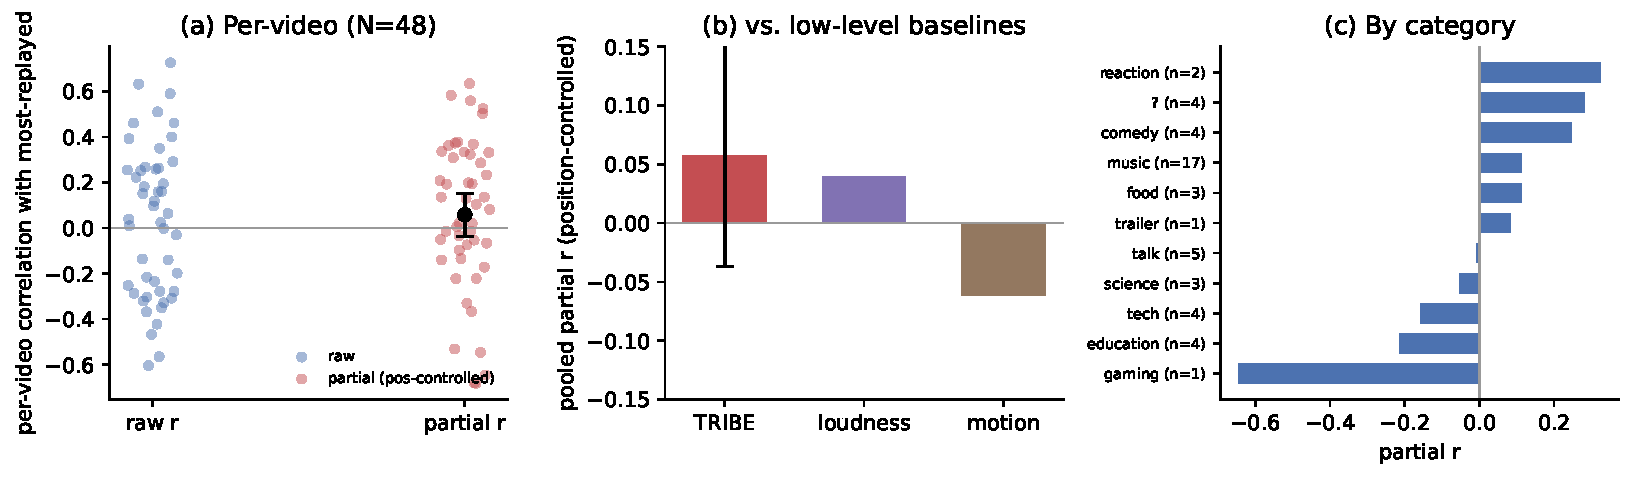
\includegraphics[width=\textwidth]{figure.pdf}
\caption{\textbf{No content-level prediction of re-watch behavior.}
(a)~Per-video raw and position-controlled correlations with most-replayed; the partial correlation
(mean $\pm$ 95\% CI) is centered on zero and the CI crosses it.
(b)~Pooled partial correlation: TRIBE is statistically indistinguishable from the loudness baseline
and near zero.
(c)~Per-category partial correlations are small, sign-inconsistent, and dominated by noise at
small $n$.}
\label{fig:main}
\end{figure}

\paragraph{Primary test.} The pooled TRIBE position-controlled partial correlation is $+0.058$
(between-video SD $=0.33$; 95\% CI $[-0.04,0.15]$), not significantly different from zero
(one-sample $t(47)=1.21$, $p=0.23$; sign test $28/48$ positive, $p=0.25$).
\paragraph{Baseline comparison.} TRIBE does not exceed the low-level baselines: the paired
difference TRIBE${}-{}$loudness ${}=0.018$ ($t=0.34$, $p=0.74$); the motion baseline is $-0.06$.
\paragraph{Raw correlation is $\approx 0$ on diverse content.} The pooled raw correlation is also
$\approx 0$ ($+0.036$). The moderate raw correlations ($0.3$--$0.8$) seen for music videos are a
genre-specific intro/onset-replay artifact that vanishes on talks, tech, science, comedy, etc.
\paragraph{Per-category.} Category-level partial correlations are small and inconsistent
(comedy $+0.25$, music $+0.11$, education $-0.21$, science $-0.05$; several $n{=}1$); no content
type shows systematic prediction.

\subsection{Video-level ranking}
The analysis above asks whether TRIBE predicts \emph{which moments} within a video are re-watched.
A complementary question is whether TRIBE ranks \emph{which videos} are more engaging overall. We
correlate video-level TRIBE summaries (mean and peak engagement) with public engagement metrics
(view and like counts) across the same $48$ videos. All associations are near zero and, if
anything, slightly negative: Spearman $\rho(\text{mean},\text{views})=-0.09$,
$\rho(\text{mean},\text{likes})=-0.14$, $\rho(\text{peak},\text{views})=-0.20$, and
$\rho(\text{mean},\text{like/view})=-0.08$ (all $|\rho|<0.28$, the $p{=}0.05$ threshold at
$n{=}48$; none significant). TRIBE engagement is thus not an indicator of video-level engagement
either. We note an important limitation: our videos are all already highly popular (views
$8\!\times\!10^4$ to $9\!\times\!10^9$, median $1.3\!\times\!10^7$), because they require a
most-replayed heatmap; this range restriction weakens the test, and a definitive virality study
would need a balanced viral-vs-flop sample.

\subsection{Region-specific readouts}\label{sec:region}
The global-field-power readout pools over the whole cortex and could dilute a signal carried by a
specific functional network, plausibly the salience/reward or sensory systems implicated in
neuroforecasting. We therefore repeated the position-controlled analysis with the engagement curve
restricted to each of five networks defined by the Destrieux atlas, recomputing GFP over only the
vertices of that network. The null is robust across all of them (pooled partial $r$, $n{\approx}48$):
whole-cortex $+0.058$, visual $-0.010$, auditory $+0.065$, salience (insula/cingulate) $+0.001$,
frontal $+0.023$, and parietal $+0.088$. The largest value (parietal) is marginal and would not
survive correction for the six readouts tested; no network approaches a level that would overturn
the whole-cortex conclusion. Spatially resolving the predicted response does not recover a
content-level re-watch signal.

\subsection{Robustness: temporal permutation}
Because both series are autocorrelated, a standard parametric test can be anti-conservative. As a
non-parametric check we recomputed the pooled partial correlation under a circular-shift null that
preserves each engagement curve's autocorrelation structure while destroying its temporal alignment
to most-replayed ($K{=}2000$ shifts, $n{=}48$ videos). The observed pooled partial $r=0.058$ falls
well within the null distribution (two-tailed $p=0.12$), consistent with the parametric test and
confirming that the near-zero effect is not an artifact of temporal autocorrelation.

\section{Discussion}
Once temporal position is controlled, TRIBE's predicted engagement has no detectable relationship
with what viewers re-watch, and it does not beat a simple loudness curve. The strong correlations a
music-only, non-position-controlled analysis would report do not generalize, which bears on the
practice of repurposing brain-encoding models as off-the-shelf engagement predictors. Several
caveats bound the claim: most-replayed is a noisy, biased behavioral target; we analyze a $60$\,s
window; and TRIBE was optimized for fMRI accuracy, not behavior. Two natural alternatives are also
ruled out here: restricting the readout to individual functional networks (including salience/reward)
does not recover a signal, and a permutation null that respects temporal autocorrelation gives the
same near-zero effect. A positive result may still require a cleaner behavioral target (view
trajectories or breakout) or a model fine-tuned for the behavioral endpoint rather than fMRI
accuracy.

\section{Conclusion}
Predicted-fMRI engagement from TRIBE does not, in this evaluation, forecast YouTube re-watch
behavior beyond temporal position and low-level audiovisual features. We release the pipeline and
encourage tests with richer readouts and behavioral targets.

\section*{Reproducibility}
Code (scoring, position-controlled validation, baselines, SABR-resilient acquisition, encoding
cache) and the list of video IDs with their most-replayed heatmaps are released with the paper.

\begin{thebibliography}{9}
\bibitem[Bardes et al.(2024)]{bardes2024vjepa} A.~Bardes, Q.~Garrido, J.~Ponce, X.~Chen,
M.~G.~Rabbat, Y.~LeCun, M.~Assran, and N.~Ballas. Revisiting feature prediction for learning visual
representations from video. \emph{arXiv:2404.08471}, 2024.
\bibitem[Berns and Moore(2012)]{berns2012neural} G.~S.~Berns and S.~E.~Moore. A neural predictor of
cultural popularity. \emph{Journal of Consumer Psychology}, 22(1):154--160, 2012.
\bibitem[d'Ascoli et al.(2025)]{dascoli2025tribe} S.~d'Ascoli, J.~Rapin, Y.~Benchetrit,
H.~Banville, and J.-R.~King. TRIBE: TRImodal Brain Encoder for whole-brain fMRI response
prediction. \emph{arXiv:2507.22229}, 2025.
\bibitem[Dmochowski et al.(2014)]{dmochowski2014audience} J.~P.~Dmochowski, M.~A.~Bezdek,
B.~P.~Abelson, J.~S.~Johnson, E.~H.~Schumacher, and L.~C.~Parra. Audience preferences are predicted
by temporal reliability of neural processing. \emph{Nature Communications}, 5:4567, 2014.
\bibitem[Genevsky et al.(2017)]{genevsky2017brain} A.~Genevsky, C.~Yoon, and B.~Knutson. When brain
beats behavior: Neuroforecasting crowdfunding outcomes. \emph{Journal of Neuroscience},
37(36):8625--8634, 2017.
\bibitem[Grattafiori et al.(2024)]{grattafiori2024llama} A.~Grattafiori et al. The Llama 3 herd of
models. \emph{arXiv:2407.21783}, 2024.
\bibitem[Hasson et al.(2004)]{hasson2004intersubject} U.~Hasson, Y.~Nir, I.~Levy, G.~Fuhrmann, and
R.~Malach. Intersubject synchronization of cortical activity during natural vision.
\emph{Science}, 303(5664):1634--1640, 2004.
\end{thebibliography}

\end{document}
